\documentclass[12pt,A4Paper]{report}
\usepackage[utf8]{inputenc}
\usepackage[a4paper,margin=1.5cm,top=2cm]{geometry}
\usepackage{graphicx}
\graphicspath{/Users/JohnnyLin/Desktop/Dzmitry_Lab /UROPS/uropsReport/figures}
\usepackage{float}
\usepackage{gensymb}
\usepackage{datetime}
\setlength{\parindent}{0pt}
\usepackage{appendix}
\usepackage{amsmath}
\usepackage[stable]{footmisc} %for footnote in title
\usepackage[hidelinks]{hyperref}
\usepackage{multirow,multicol}
\usepackage{adjustbox}
\usepackage{fancyhdr}
\usepackage{parskip}
\usepackage{caption}
\usepackage{listings}
\pagestyle{fancy}
% \fancyhf{}
\rhead{UROPS-CQT}
\lhead{Lin Zhonglin A0222183N}

\title{UROPS Report}
\author{Lin Zhonglin \hspace{1cm} A0222183N}
\usdate{}

\begin{document}
\maketitle

\section{Introduction}
Craft a short text that links up all section of my report. Possibily linking to the main ion trapping expt in lab. 

\section{Building and tuning a compact 638nm Grating Stabilized Diode Laser}
Since their first use in atomic physics in the early 80's, diode lasers have become an important part of many modern experiments. This is primarily due to the high reliability and the low price of these devices which facilitate experiments involving a number of lasers operating at different frequencies \cite{compactGratingDiodeLaser}.
\par
This section of the report discusses a type of compact grating-grating stabilized diode laser system. There was a constructed 638nm laser system of this type in the lab with a dead diode. I replaced the diode and tuned the laser back to 638.....nm wavelength for probing of one of the Ytterbium ion state. 
%TODO: search up on the exact frequency and discuss how it's used in the lab
\par
Resources relevant to this task: 
\begin{enumerate}
    \item book - Principles of Lasers \cite{principleOfLasersOrazio}: Chapter 9 discusses semiconductor lasers. Chapter 4.7 discusses Gaussian Beam Optics. 
    \item paper - A compact grating-stabilized diode laser system for atomic physics \cite{compactGratingDiodeLaser}: This paper discusses the detailed mechanical design and construction process of one of the most commonly used diode lasers in optics labs, with linewidth of a few 100kHz. 
\end{enumerate}

%TODO: insert the laser setup image here: both schematic and the real thing

Although a free-running diode suffers from large linewidth, an optical cavity that provides optical feedback can greatly reduce its linewidth. In the system under discussion, first order light diffracted light from a grating is coupled back into the diode, so that the grating and the diode's facet form an external resonator. The use of a grating results in a linewidth reduction of two orders of magnitude and it also allows the selection of any desired wavelength. The external cavity length (distance between grating and diode) is chosen to be about 15mm optimise for single mode operation. A peltier element is embedded in the mechanical structure to maintain temperature of the system. A piezo actuator is embedded behind the grating to allow small adjustment and scan of the external cavity length. (See \cite{compactGratingDiodeLaser} for more details)
\par
To tune the emission wavelength of this laser, consider the following rough picture. The gain profile of such laser diode has a typical width of 10nm. The emission wavelength is determined by the competition between the longitudinal modes of the laser cavity, which are typically separated by 100-200 GHz. The laser operates at the mode which experiences the maximum gain (See Fig \ref{fig:diodeLaserGainCurve}.
\begin{figure}[H]
    \centering
    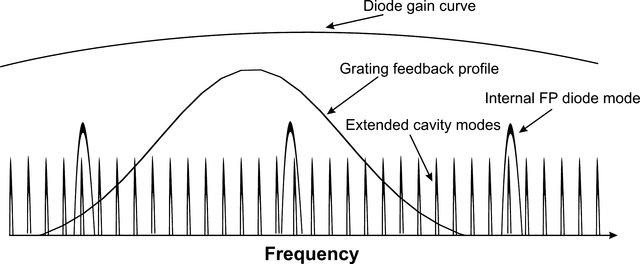
\includegraphics[width=.8\textwidth]{diodeLaserGainCurve.jpg}
    \caption{Laser Diode Gain Profile}
    \label{fig:diodeLaserGainCurve}
\end{figure}
Hence there are two main ways of tuning the emmision wavelength, tuning the temperature or the injection current: \cite{compactGratingDiodeLaser}. 
\begin{enumerate}
    \item Temperature variations cause a change of the cavity length (and thus a change of the resonance frequencies of the longitudinal modes) and at the same time a frequency shift of the gain profile. Consequently, the emission wavelength can be tuned with the temperature. However, in the process of tuning, the gain of the modes varies such that at some point the laser eission frequency jumps from one mode to another (commonly referred to as \textbf{mod-hopping}), resulting in a number of inaccessible frequency domains. \cite{compactGratingDiodeLaser} suggests that the width of the accessible frequency domain is typically a fraction of the spectral range of the laser cavity. Here with laser cavity being 15mm, it's several tens of GHz.

    \item A second method which can be employed to tune the emission wavelength is to vary the injection current. This leads to a corresponding temperature change and also a change of the carrier density and thus of refractive index of the semiconductor material. Injection current tuning also suffers from mode hopping. 
    \par
    Note: Temperature tuning can cover a frequency range of the order of several tens of nm in wavelength at a typical rate of 0.3 nm/K, injection current typically covers a range of several tens of GHz only at a typical rate of 4GHz/mA. 
\end{enumerate}
 
After careful replacement of the original dead diode, coarse adjustment of the wavelength is achieved by horizontally tilting the grating with the micrometer screw. The main goal now is to vary the temperature and injection current in search for a mode-hopping-free region in the gain profile near the desired wavelength of around 638.615nm. Fig \ref{fig:diodeLaserEW} shows a few tens of data points of temperature-EW plots. The bottom data points from a dense grid as expected, showing that it's a mode-hop-free region. Whereas the top few data points probably is a result of mode hopping. After many trial and error, the final set of parameters arriving at EW=638.615nm is [set temperature for the peltier = 17.92$\degree$, set current = 52.3mA, current offset = -0.563 mA, piezo voltage = 2.5 V] However, this EW still suffers from drifting. 
%TODO: explain the current offset here

\begin{figure}[H]
    \centering
    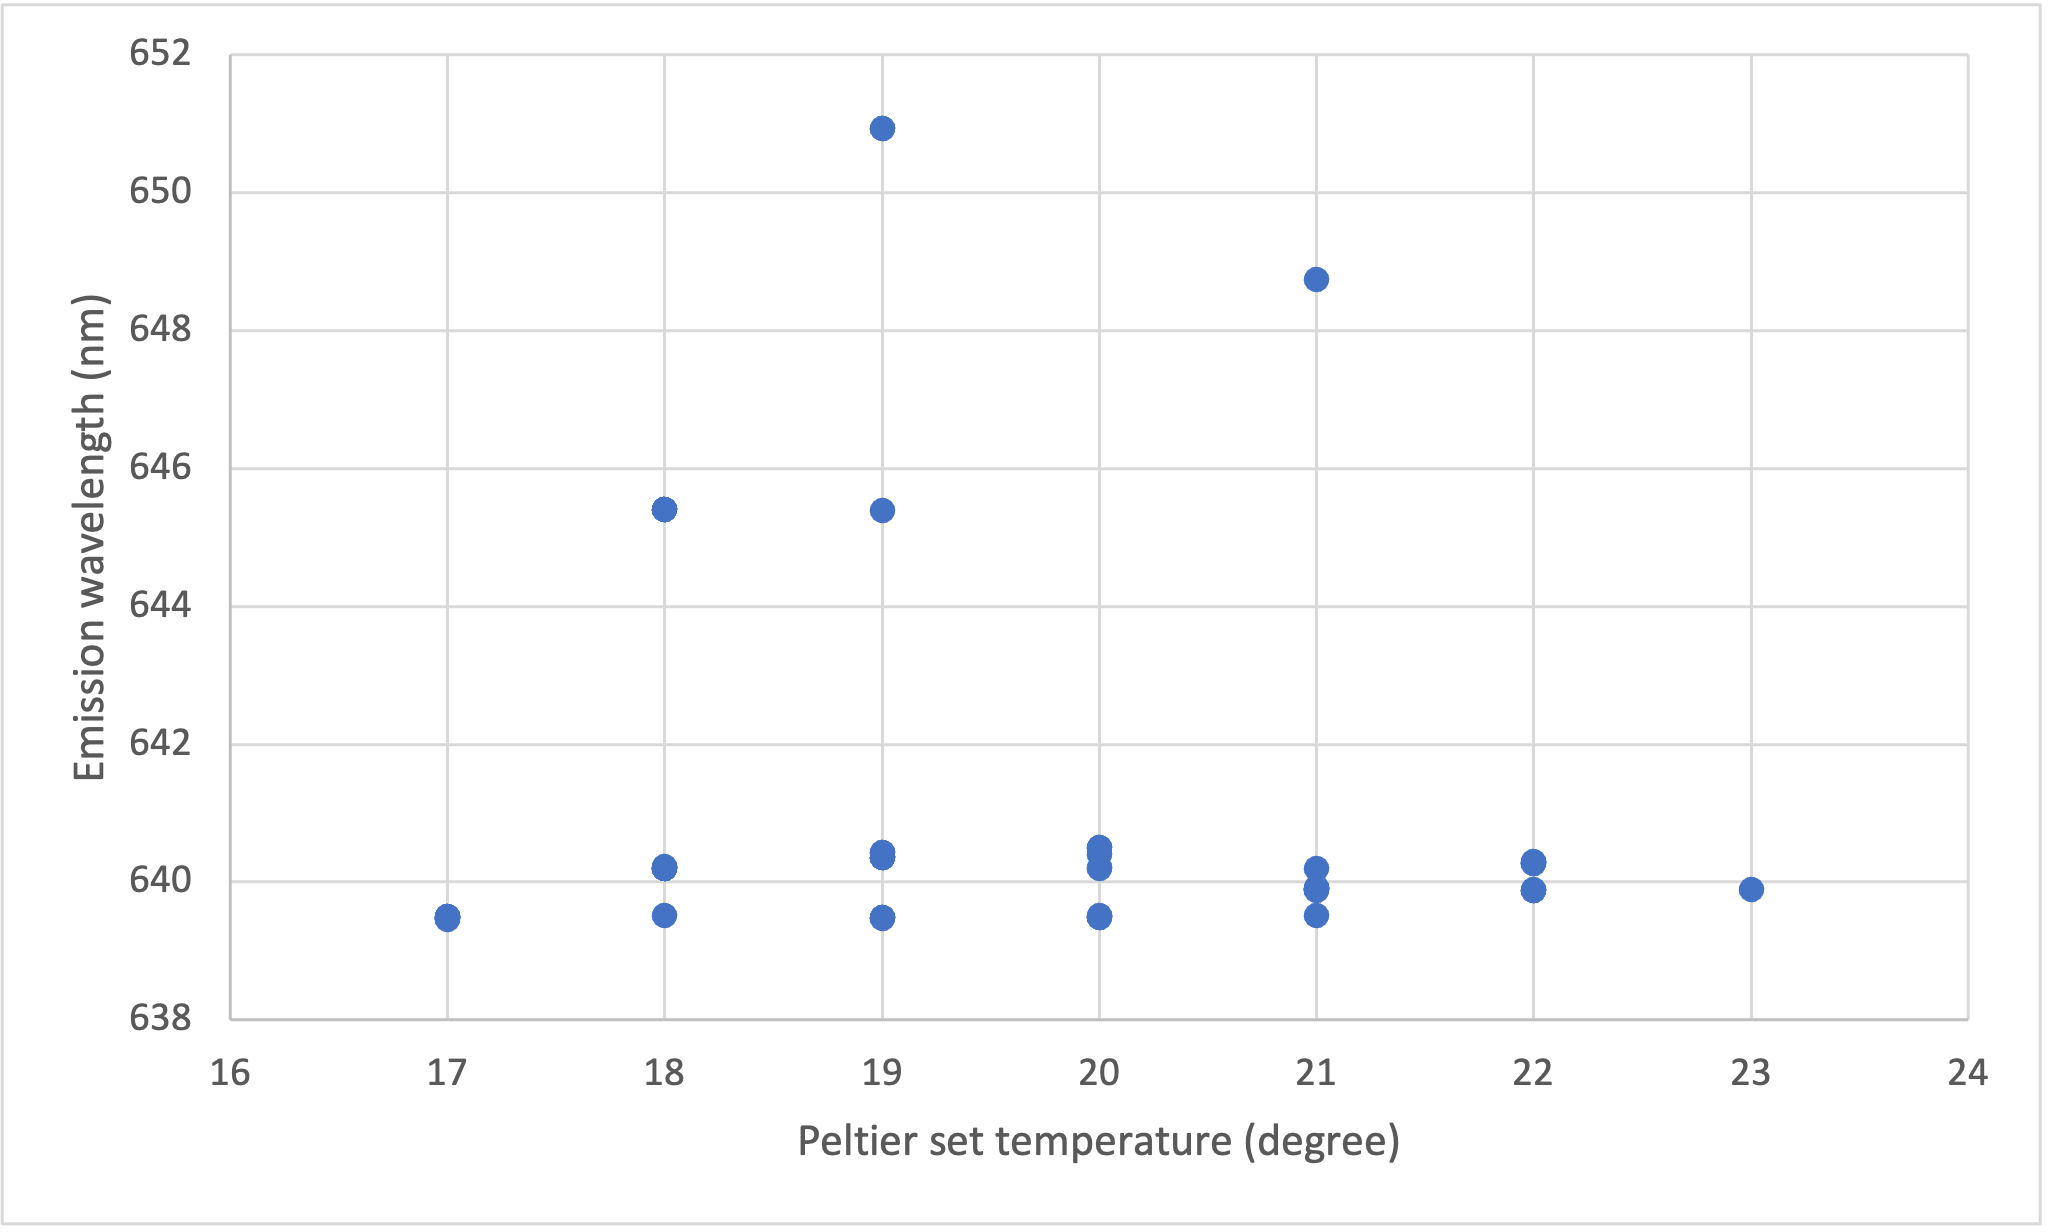
\includegraphics{diodeLaserEW.png}
    \caption{Diode EW - temperature}
    \label{fig:diodeLaserEW}
\end{figure}
\subsection{Gaussian Beam Characterisation and collimation}
%TODO: add some gaussian beam theory here
When dealing with laser beams, Gaussian beam optics is commonly considered. As the laser diode has a rectangular shape, its initial output laser beam has an oval shape and thus not very Gaussian and not very suitable for subsequent Gaussian beam characterisation and coupling to optical fibres. A pair of anamorphic prism is first used to tune the laser beam cross section to be as circular as possible. (See Fig...) Next it's desirable to collimate the beam for ease of coupling into other optical components. Coarse collimation can be done by eyeballing the change of the beam spot diameter at different distance from the collimating lens and adjusting the position of the collimating lens to make beam spot diameter as constant as possible across the scanning distance. To achieve finer collimation, consider the following Gaussian beam characterisation process: 
\begin{enumerate}
    \item First we need to measure the beam spot diameter at different distances from the collimating lens. To do so, consider the knife edge measurement for very precise measurement. Alternatively consider using a CCD camera for measurement for precision of up to $\mu m$ level precision. 
    \begin{enumerate}
        \item knife edge measurement: %TODO: explain and import code here
        \item camera measurement: %TODO: explain and import code here
    \end{enumerate}

    \item After measuring the beam diameter at as many differnt distances as possible, fit the data to the Gaussian beam beam radius - z posisiton by using the code ... in Annex to arrive on estimation of the beam waist radius and z position. Adjust the collimating lens accordingly to make the beam waist z position as far as possible. 
\end{enumerate}
\subsection{Laser beam - Fiber Coupling Procedure}
%TODO: put a picture of the set up here
In order to monitor the laser system emission wavelength, part of the laser beam power is sent to the wavemeter via a fiber. To send a laser beam into a single-mode optical fibre is to couple their spatial modes, follow this procedure for coupling optimisation: 
\begin{enumerate}
    \item Make sure that the laser beam at least go through one mirror before being sent to the fibre mount to allow for two points of freedom. Rough align the collimated beam through the fiber mount without the fibre on. Try to center the beam through the fibre mount entry. 
    \item Screw optical fiber onto the fiber mount and attach a fiber testing pen to the exit end of the fibre. Place a piece of paper on the optical path and try to align the two spots from the diode laser and the fibre pen by iteratively adjusting the mirror and the fiber mount. 
    \item Detach the fibre pen and sent the light from the exit end of the fibre (if no light at all, go back to previous step) to a power meter and perform "Walking-the-beam" technique \cite{WalkingTheBeamThorlabs} to optimise coupling. 
    \item If the previous step doesn't go to efficiency above 50\%, turn the fiber mount lens position to optimise. Note that this is very sensitive, so adjust the fibre mount lens with small turns of about 2-3$\degree$ at a time. As the optimised position is approached, even finer adjustment is required. 
    \item Note that coupling efficiency above 60\% requires significantly more effort than described. More sophisticated techniques need to be employed. However, this methods should lead to a minimum of 60\% coupling, if not achievable consider: 
    \begin{enumerate}
        \item Clean the optics: fibre cross section and mirrors.
        \item Check whether the fibre has any leakage by using a fibre pen and look for light leakage in a dark room. 
        \item Consider tuning in a larger range to get out of a possible local maximum. 
    \end{enumerate}
\end{enumerate}

\section{EOM (Electro-optic Modulator)}
% put basic intro to an EOM here 
In certain types of crystals it is possible to effect a change in the index of refraction that is proportional to the applied electric field. This is the linear electro-opic effect (also known as the Pockels effect). Applying a modulated electric field across such a nonlinear crystal (usualy the KDP type) and passing a beam of laser through the crystal leads to the laser beam being modulated in phase. (detail see: \cite{fundamentalsOfPhotonics}

\subsection{Theory and Model}
When a time-varying electric field is applied to the nonlinear crystal inside the EOM, the index of refraction $n$ changes in a sinusoidal manner resulting in phase modulation of the laser beam passing through the crystal. Consider the following short mathematical example to see that phase modulation is equivalent to frequency: 
\\
% 见激光原理for this part
Suppose instantaneous electric field at a point of EM wave of a laser beam: 
\begin{align*}
    E_c(t) = A_c cos(\omega_c T + \varphi_c)
\end{align*}
With phase modulation (assume sinusoidal modulation), we have final phase of the electric field of the EM wave: 
\begin{align*}
    \psi(t) &= \omega_c t + \varphi_c + \Delta \varphi (t) \\
            &= \omega_c t + \varphi_c + m_{\varphi} sin(\omega_m t)
\end{align*}
So the modulated electric field now becomes: 
\begin{align}
    E(t) &= A_c cos[ \omega_c t + m_{\varphi} sin(\omega_m t) + \varphi_c] \label{eqn:7.1.9}\\
         &= A_c cos\left\{  \int_0^t [ \omega_c + \Delta ]\omega(t)] dt + \varphi_c \right\} \\
\end{align}
where, 
\begin{equation*}
    \Delta \omega (t) = \frac{d\Delta \varphi (t)}{dt}
\end{equation*}
If we do Fourier transform to Eqn \ref{eqn:7.1.9}, we obtain in frequency space: 
\begin{equation}
    E(\omega) = A_c J_0(m) \delta(\omega - \omega_c) + A_c\sum_{n=1}^\infty J_m(m) \left\{ \delta[\omega-(\omega_c + n\omega_m)] +(-1)^n\delta[\omega-(\omega_c-n\omega_m)]\right\}
    \label{eqn:7.1.10}
\end{equation}

Eqn \ref{eqn:7.1.10} shows that when a single-frequency laser beam is modulated by a sinusoidal frequency, the modulated beam in frequency space comprises of the unmodulated frequency $\omega_0$ and infinite sidebands. Sideband frequency spacing is $\omega_m$, modulation frequency. 
% actually not sure about this, need to double check the math
Sideband amplitudes are determined by the Bessel function $J_n(m)$. (See Fig \ref{fig:EOMsidebandTheory}) What's of concern in this case is that EOM phase modulation produces frequency sidebands of laser beam. 

\begin{figure}[H]
    \centering
    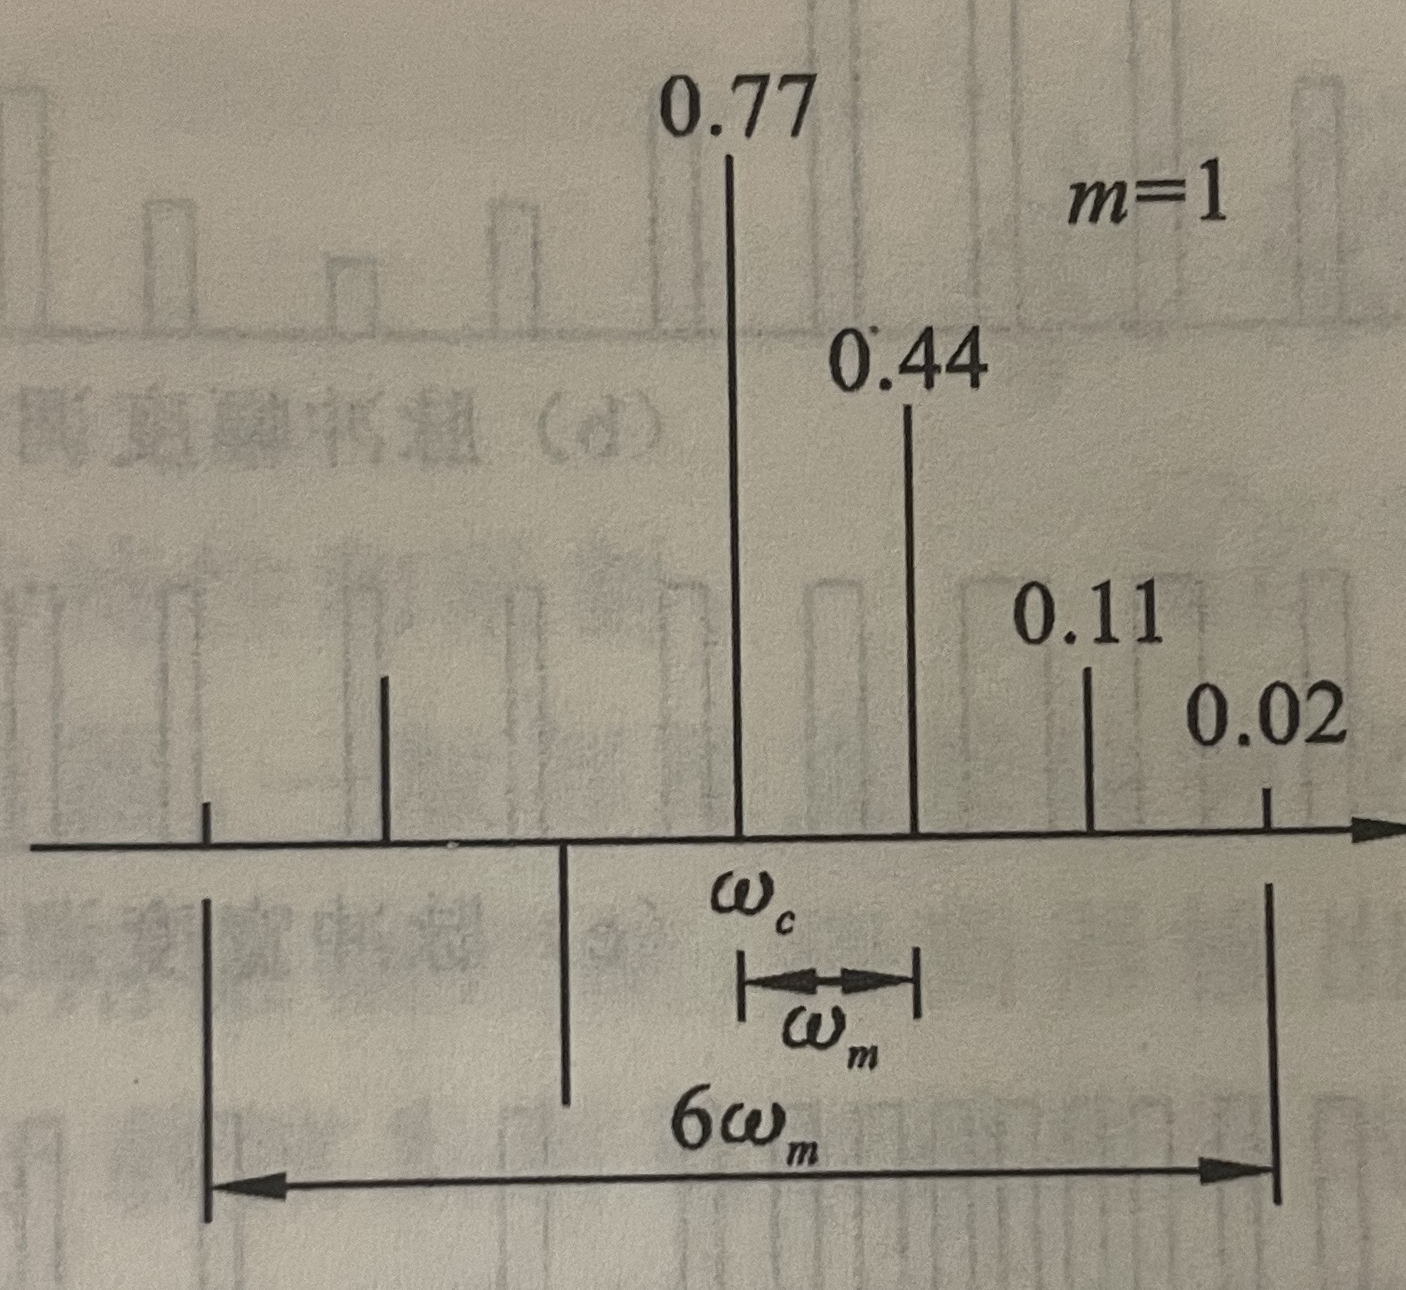
\includegraphics[width=0.3\textwidth]{EOMsidebandTheory.png}
    \caption{modulated laser beam frequency sepctrum}
    \label{fig:EOMsidebandTheory}
\end{figure}

 \subsection{EOM Tank Circuit Board: Model and Construction}
To construct an EOM tank circuit board and tune it to a partiular frequency, the following sources are useful: 
\begin{enumerate}
    \item paper: Design and construction of an efficient electro-optic modulator for laser spectroscopy\cite{20MHzEOM}
    \item textbook: Fundamentals of Photonics\cite{fundamentalsOfPhotonics}
    \item Prof Christian group's internal wiki has an entry on "How to build an EOM". There is a set of detailed note on EOM construction written by Meng Khoon. 
\end{enumerate}
The schematic of EOM circuit board is shown in Fig \ref{fig:eom-tank-cirucuit1}. Note that the components L, $C_1$, $C_2$ are nonideal components, i.e. the parasitics are if gnored here.
$C_1$ refers to EOM crystal (ideally with correct AR coating for the relevant wavelength, in my case $\approx$738nm and $\approx$965nm)

\begin{figure}[H]
    \centering
    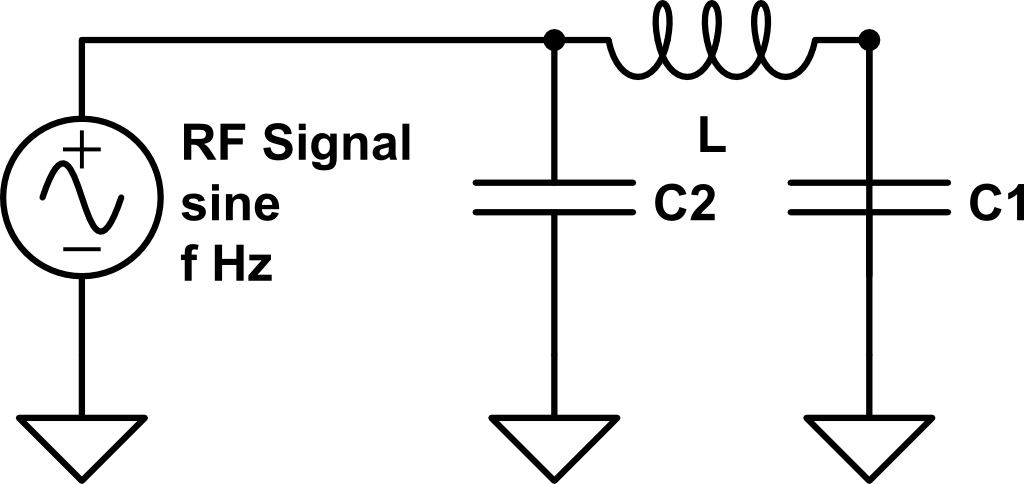
\includegraphics[width=.5\textwidth]{eom-tank-cirucuit1.png}
    \caption{EOM tank circuit board schematic (non-ideal component)}
    \label{fig:eom-tank-cirucuit1}
\end{figure}

The task of constructing an EOM at a particular modulation frequency can be be roughly be broken into the following three steps:
\par
Firstly, the LC circuit is in place to act as an amplifier so that the EOM can driven with low-power RF source of $<$ 1W, yet still providing significant electric field across the crystal for phase modulation. 
\par
Since we have an intended EOM modulation frequency frequency $f_0$, and the capacitance of the EOM crystal $C_1$ is fixed, we need to measure $C_2$ in order to backcalculate the inductor $L$ needed. Since the capacitor is small at the $pF$ level, we need to characterise $C_1$ by hooking it up with a suitable resistor, sending a square wave through it and determine its response time. Although the capacitance of the crystal should be predominantly determined by the crystal dielectric, my observation showed that the way that it's glued to the tank circuit also affects. I used silver containing glue spreaded evenly under the crystal and attached the crystal to the EOM tank circuit board's exposed copper section. The conductive glue is such that bottom of the crystal has a common ground hence electric field across the crystal will be near homogeneous as wanted. For my crystal with the way that it was glued, $C_1 \approx 3 \mu F$.
%TODO: insert measurements of crystal capacitance here
\par
After measurement of $C_1$, we can estimate the capacitance of the tank circuit board to be $C' = \frac{C_1C_2}{C_1+C_2} \approx C_1$. This is because $C_1 \gg C_2$ where $C_2$ is a coupling capacitor that will be explained later. The resonant frequency of the tank circuit can be estimated to be $f = \frac{\omega}{2\pi} = \frac{1}{2\pi\sqrt{LC'^2}}$. Rearranging to get $L = \frac{1}{(2\pi f C_1)^2}$, to get a resonant frequency of about 35 MHz, a $2 \mu H$ inductor is needed, the closest off-the-shelf inductor is $2.2 \mu H$. 
\par
Next the overall impedance of the EOM tank circuit needs to be matched to be $50\ohm$ such such that RF signal going to the EOM tank will be mostly absorbed and not reflected. In order tune the overall impedance of the EOM tank circuit, a coupling capacitor $C_2$ is added as shown in schematic \ref{fig:eom-tank-cirucuit1}. The overall loss of the EOM tank circuit can be modelled by a resistor $R_p$ as shown in Fig \ref{fig:eom-tank-cirucuit2}. Here we consider the components ideal. Note that parasitic resistance can be dependent on signal frequency, environment and many others. Here take it as $ R_p \approx 15 \Ohm$ based on Meng Khoon's note. However, much more careful characterisations of the circuit can be done. The coupling capacitor does not affect the tank circuit resonant frequency significantly as $C_1 \gg C_2$. so $C' = \frac{C_1C_2}{C_1+C_2} \approx C_1$ as mentioned earlier.  

\begin{figure}[H]
    \centering
    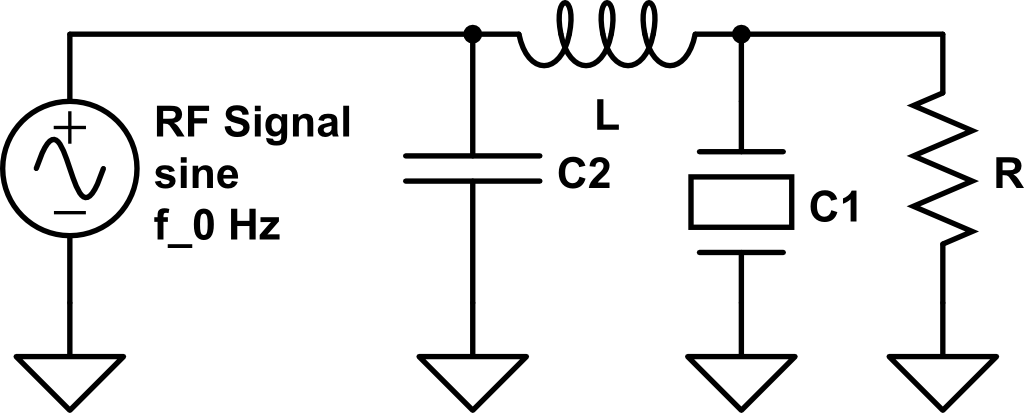
\includegraphics[width=.8\textwidth]{eom-tank-cirucuit2.png}
    \caption{EOM tank circuit, modelling overall loss}
    \label{fig:eom-tank-cirucuit2}
\end{figure}

We can calculate the overall impedance of the circuit based on this model. Setting overall impedance to be $50\Ohm$, the needed $C_2$ can be backcalculated to be $C_2 = \frac{\sqrt{50/R_p -1}}{50} \approx 93.8 nF$ which is indeed much smaller than $C_1 \approx 3 \mu F$. Choose a variable capacitor around this range of capacitance. 
\par
Lastly set up a measurement circuit as shown in Fig \ref{fig:eom-freq-measurement-setup.png}. Tune the variable capacitor until reflected signal from the EOM tank circuit board is minimum. Note that most variable capacitor has a tuning range of less than $360\degree$, so tune slowly until the valley shown on the spectrum analyser is the deepest. 

\begin{figure}[H]
    \centering
    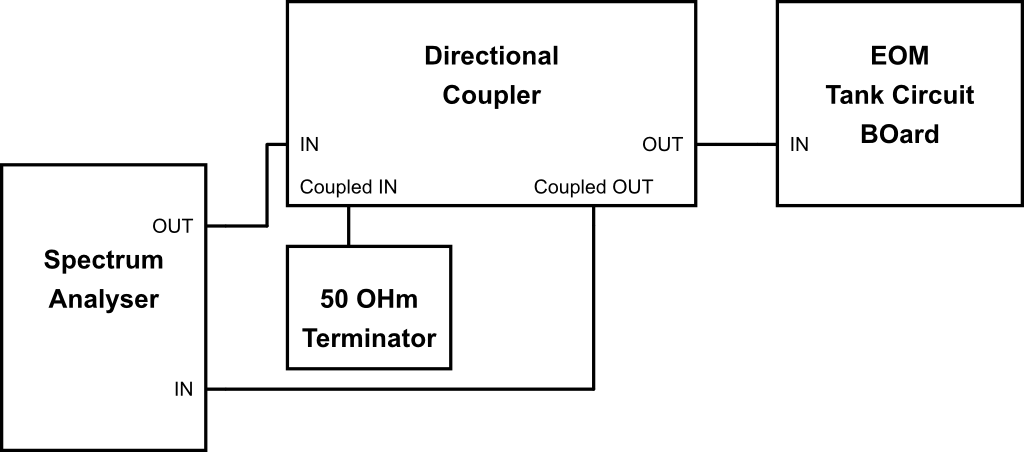
\includegraphics[width=0.8\textwidth]{eom-freq-measurement-setup.png}
    \caption{EOM frequency measurement setup}
    \label{fig:eom-freq-measurement-setup.png}
\end{figure}

After tuning the variable capacitor, my EOM tank circuit board has a resonant frequency $f_0 \approx 38 MHz$, see Fig \ref{fig:EOMfrequencyMeasurement}. 

\begin{figure}[H]
    \centering
    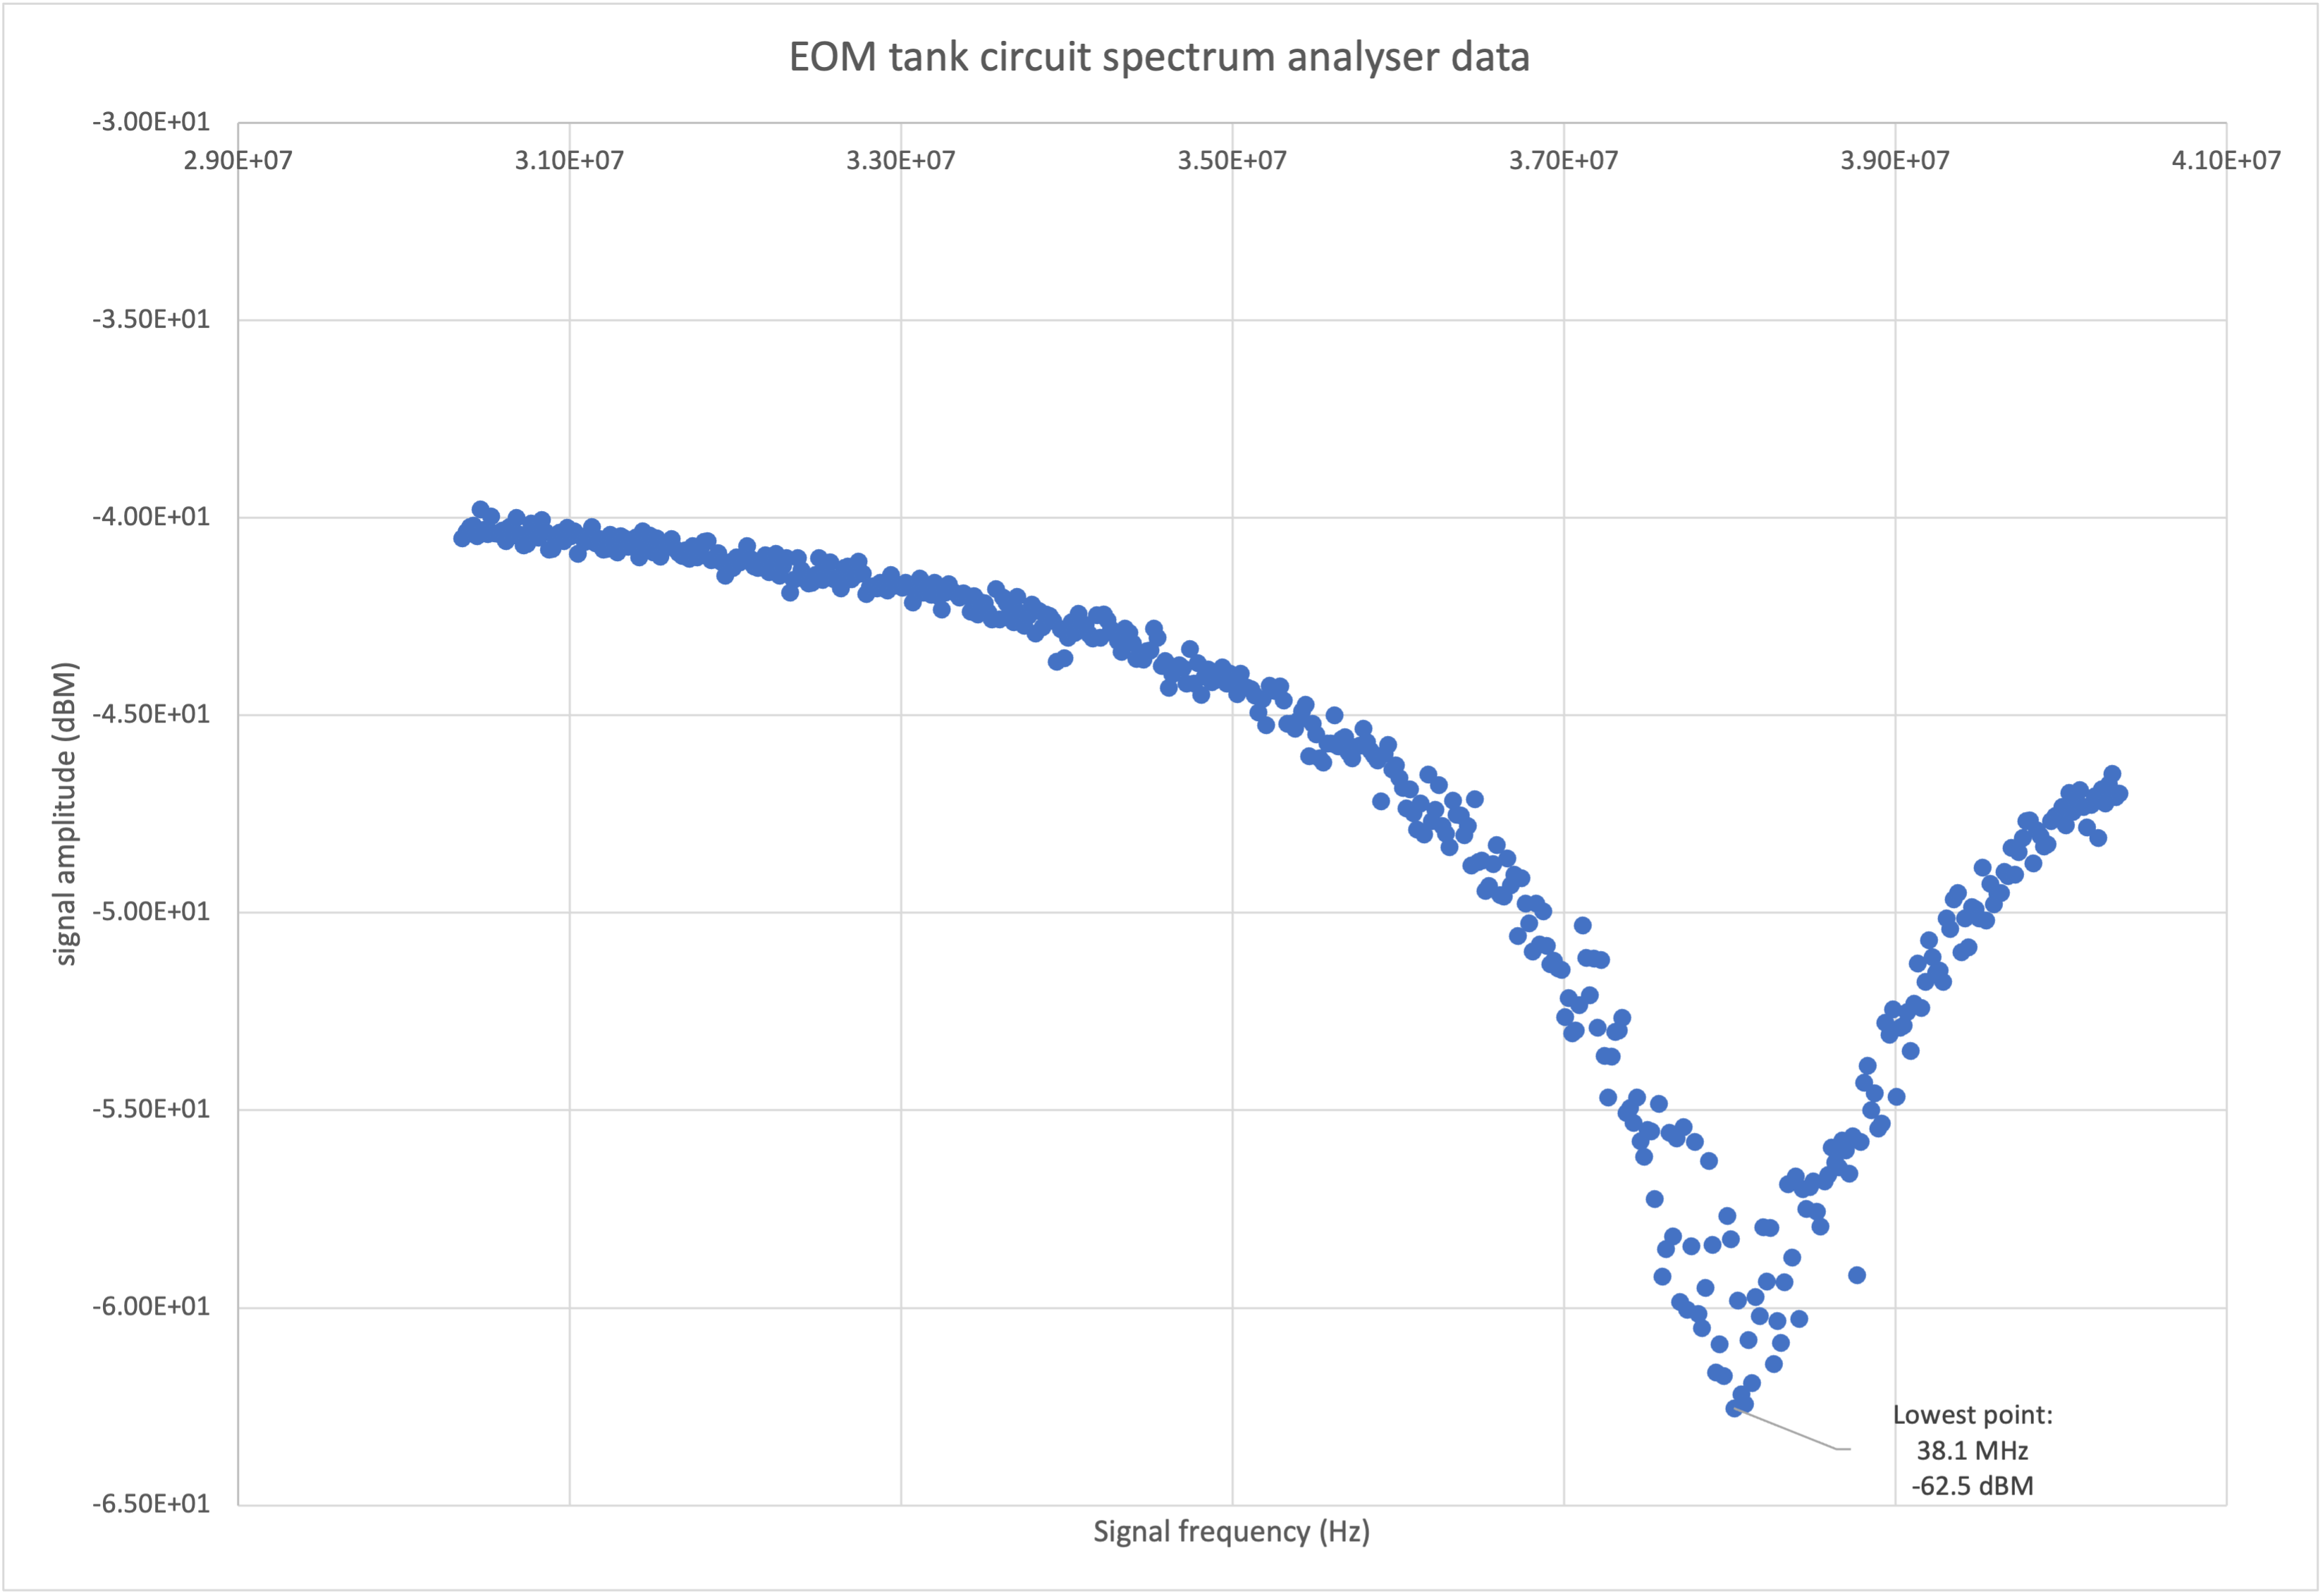
\includegraphics[width=0.8\textwidth]{EOMfrequencyMeasurement.png}
    \caption{EOM tank circuit frequency measurement setup}
    \label{fig:EOMfrequencyMeasurement}
\end{figure}

A final word on EOM construction: To improve on the Q-factor of the EOM tank circuit, parasitics of the circuit need to be better charactersied and subsequently matching impedance better. A better impedance matching will lead to higher efficiency of absorption of input RF signal. A small-voltage RF signal can bring about more significant modulation. However, my EOM as it currently is suffices for my subsequent task. 
%TODO: measure Q-factor of my EOM board
%TODO: insert an image of my actual EOM board here

\section{Fabry-Perot Cavity}
Laser resonators are open structures containing two or more mirrors that are aligned to produce optical feedback to the gain element. In the simplest case, a resonator consists of two aligned mirrors. These mirrors are called end mirrors and define the optical cavity. Optical radiation circulates within the cavity, bouncing back and forth between the end mirrors and passing through the gain element. An optical resonator can be characterised by the following parameters: 
\begin{enumerate}
    \item number of mirrors constituting the resonator
    \item focal length of mirrors
    \item radius of mirrors (usually small relative to cavity length)
    \item length of cavity
    \item reflectivity of mirrors
    \item other optical losses: how good is the vacuum in the cavity and so on
\end{enumerate}
What's relevant to this report is a particular type of optical resonator: confocal Fabry-Perot cavity. Fabry-Perot cavities are optical cavities with two parallel mirrors. Confocal Fabry-Perot cavities have focal points of the two concave mirrors overlapping at the center of the cavity as shown in Fig \ref{fig:confocalCavity}. The confocal cavity I used in experiment has a cavity length of L=15cm. 

\begin{figure}[H]
    \centering
    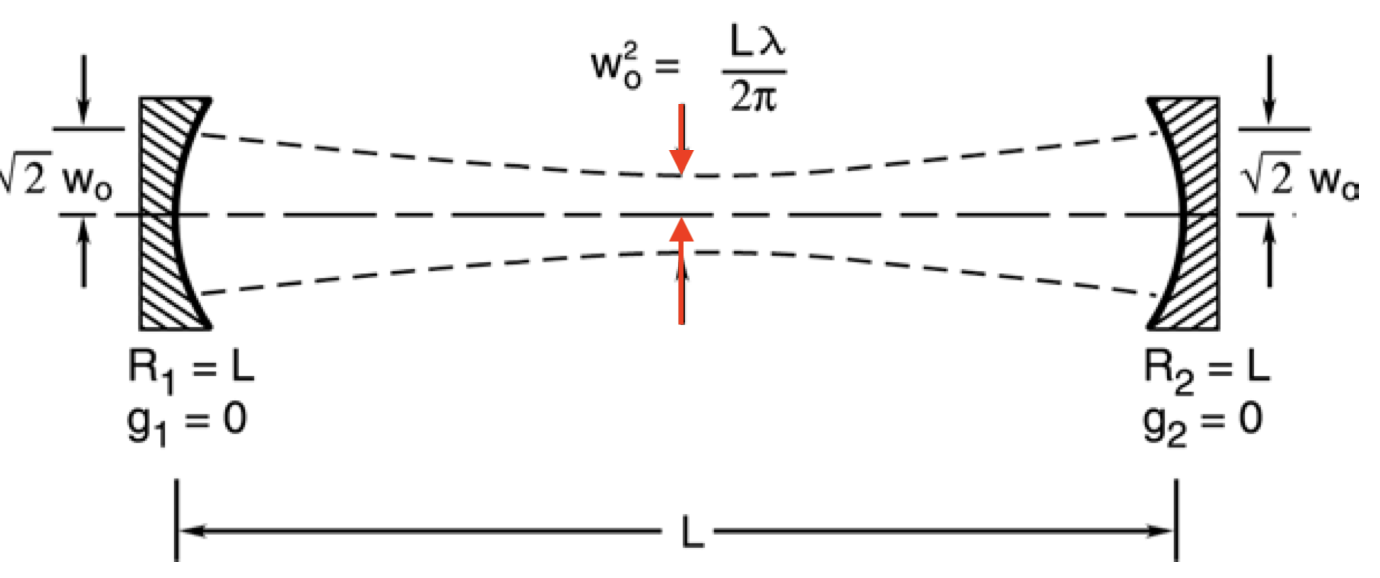
\includegraphics[width = .8\textwidth]{confocalCavity.png}
    \caption{Confocal cavity}
    \label{fig:confocalCavity}
\end{figure}

One good way to measure the frequency of a laser's beam is send it into a Fabry-Perot cavity and look at what gets transmitted (or reflected). Light can only pass through a Fabry-Perot cavity if twice the length of the cavity is equal to an integer number of wavelengths of the light. Or equivalently put, the frequency of the light's electromagnetic wave must be an integer number times the cavity's free spectral range $\Delta \nu_{fsr} \equiv c/2L$, where $L$ is the length of the cavity and $c$ is the speed of light. For my case $\Delta \nu_{fsr} \approx 1GHz$. The cavity acts as a filter, with transmission lines, or resonances, spaced evenly in frequency every free spectral range. Fig \ref{fig:cavityTransmission}  shows a plot of the fraction of light transmitted through a Fabry-Perot cavity versus the frequency of the light. \cite{PDHintro}\cite{fundamentalsOfPhotonics}

\begin{figure}[H]
    \centering
    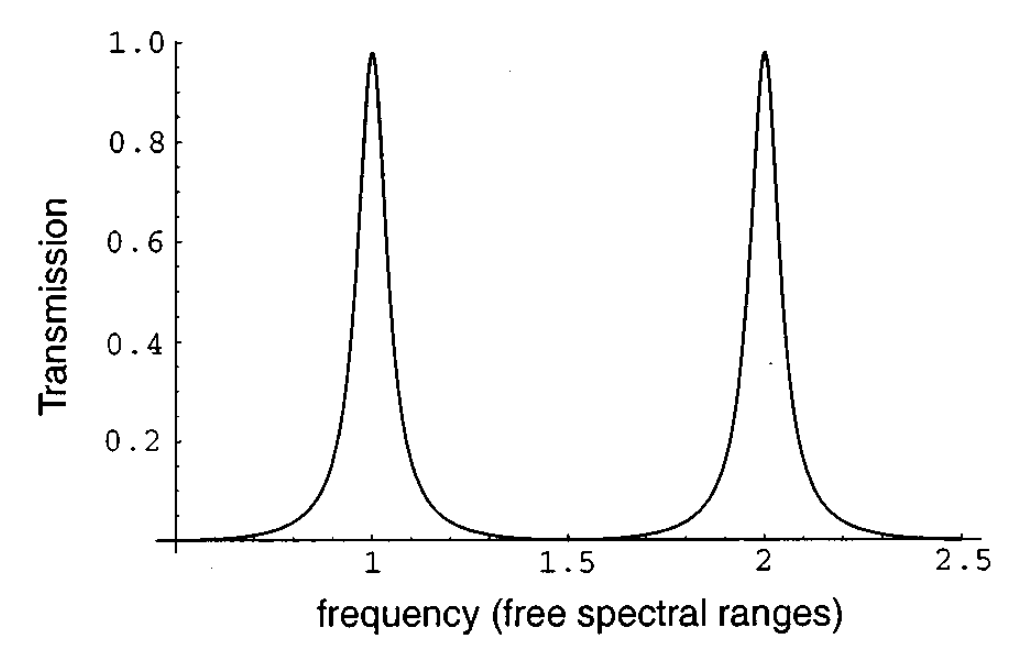
\includegraphics[width=.8\textwidth]{cavityTransmission.png}
    \caption{Cavity transmission}
    \label{fig:cavityTransmission}
\end{figure}

\subsection{Laser beam - Cavity Coupling}
To couple a well collimated laser beam with beam radius $\omega_1$ (see section on laser beam collimation and characterisation in this report) into a Fabry-Perot cavity, follow these steps: 
\begin{enumerate}
    \item Choose a thin lens (with relevant AR coating) of focal length $f$ to focus the laser beam from radius $\omega_1$ to $\omega_0$ at the center of the cavity. Gaussian beams have a propagating spherical wavefront, and each Gaussian beam is uniquely characterised by its beam waist, here being $\omega_0$. In the context of a confocal cavity, when a Gaussian has beam waist $\omega_0 = \frac{L\lambda}{2\pi}$ as shown in Fig \ref{fig:confocalCavity} the Gaussian beam spherical wavefront at the mirrors will match the curvatures of the mirrors, hence leading to stable standing waves to establish in the cavity. In my case, consider $L=15$ cm, $\lambda = 935.18848$ nm,  $\omega_0$ = $0.000149419$ m.
    
    \item To determine the focal length $f$, we consider how parameters of a Gaussian beam transforms through a thin convex lens (see \cite{principleOfLasersOrazio} for details). Approximately, we have $\omega' \approx \frac{\lambda f}{\pi \omega}$. Where, $\omega'$ is the 'image'-side beam waist, $\omega$ is the 'object'-side beam waist, $\lambda$ is laser beam wavelength, $f$ is the thin lens focal length. In my case, consider $\lambda = 935.18848$ nm, $\omega'$ = $0.000149419$ m. $\omega = 1.1$ mm (image-side beam radius is estimated to be so through beam characterisation) $f = frac{\omega' \pi \omega_1}{\lambda} \approx 0.552139m \approx 550mm$. However, using a lens of such focal length was not practical due to space constraint on the optical table, I used a $f=150mm$ thin lens as it was the longest focal length lens available off-the-shelf. 
    
    \item Pass the laser beam through at least one mirror before entering the cavity to obtain at least 2 points of adjustment. See Fig \ref{fig:laserCavityCoupling} in Appendix for a hand-written note on how to adjust the mirrors (or fibre mount) for optical coupling using a card (either normal paper or IR paper depending on wavelength) with a hole. 

    \item Lastly send a triangle wave signal of appropriate $V_{pp}$ to the piezo actuator to scan the cavity length across a certain range. The $V_{pp}$ needed depends on the scanning range needed and the behaviour of the piezo actuator. See chapter 2 of \cite{FundamentalPrinciplesofEngineeringNanometrology} for details on piezo actuators. For my case, after testing, a triangle wave generator board producing $\pm 5$V, together with a voltage gain board of coefficient 19 is used to produce a $V_{pp} \approx 190$V. See Fig \ref{fig:935cavityScan}, yellow line comes from a sync port of the triangle wave generator, green line comes from a photodiode at the exit end of cavity. Notice that "half a triangle" covers two peaks (not optimised in this image, but it was optimised after the image was taken), indicating that the cavity scan range is sufficient to cover a free spectral range of my cavity. Fine tune the cavity to obtain highest peaks possible 
    \par
    Caution: 
    \begin{enumerate}
        \item The piezo actuator might fracture under high negative voltage, so avoid sending in negative voltage to it. For my case, I used a offset gain baord to make sure the triangle wave sits above 0V.
        \item The voltage sent to the piezo actuator is HV, be cautious and remember to electrically insulate the cavity from the optical table.
    \end{enumerate}
\end{enumerate}

\begin{figure}[H]
    \centering
    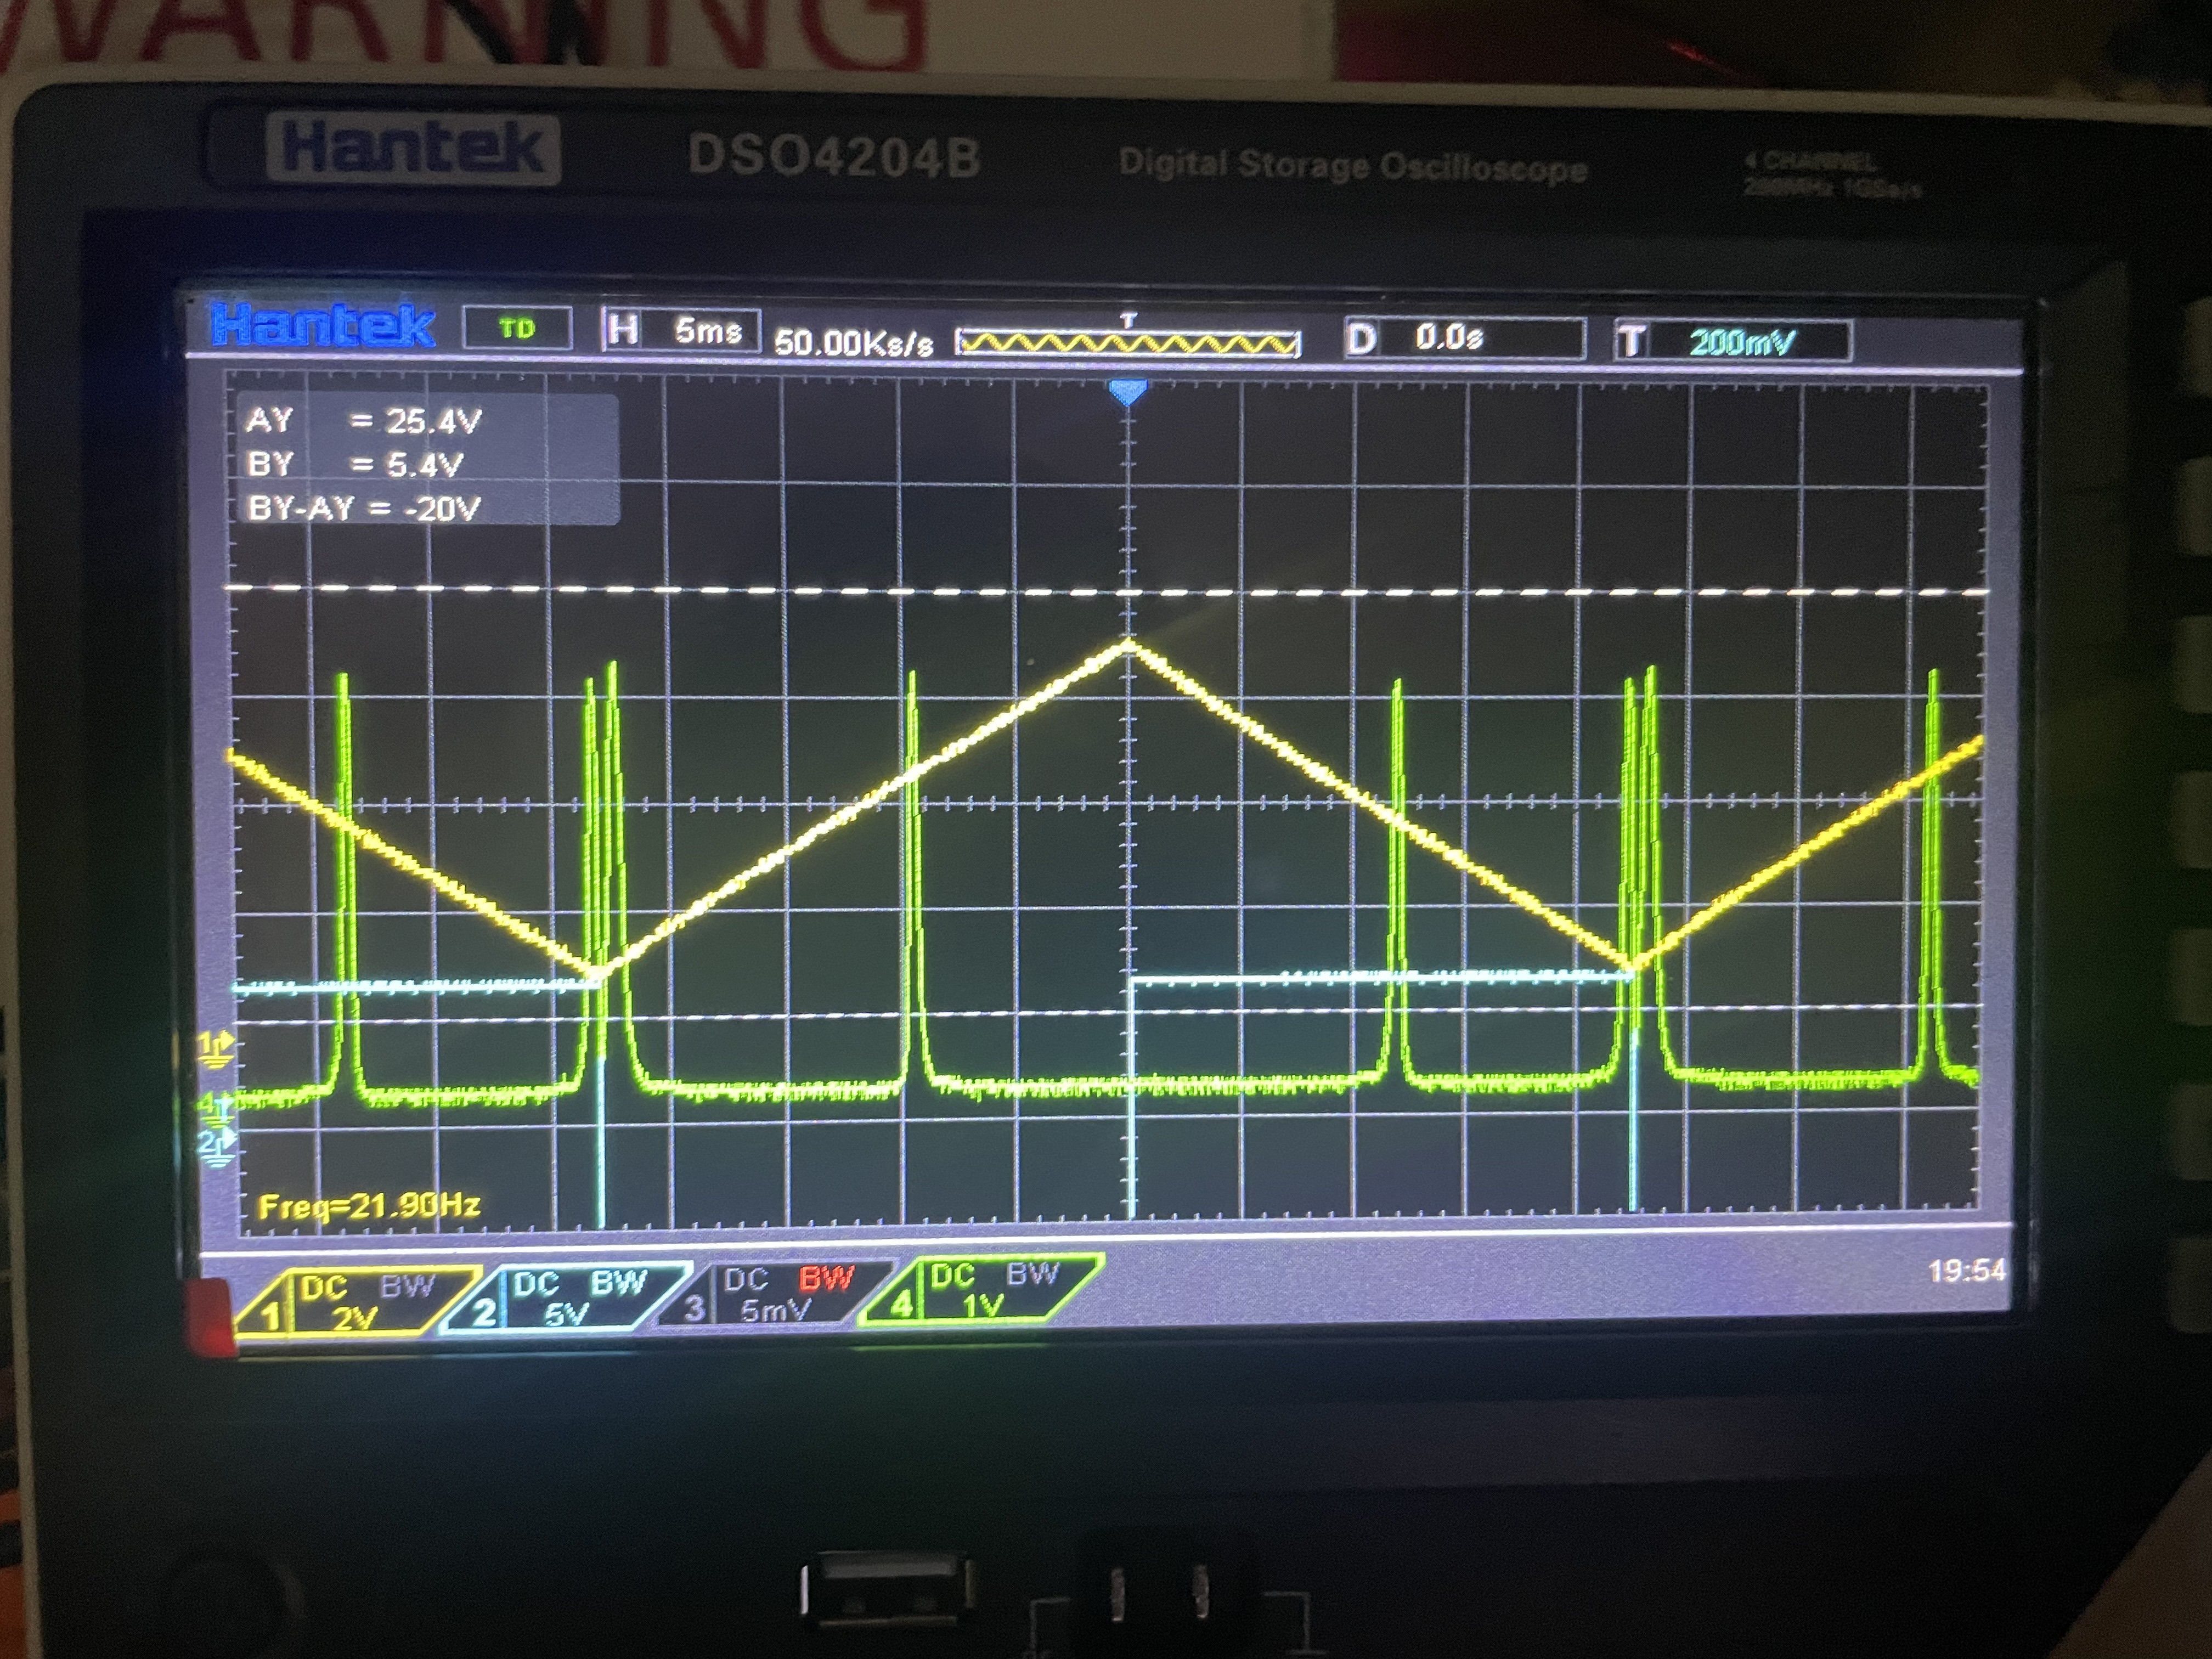
\includegraphics[width=.8\textwidth]{935cavityScan.jpeg}
    \caption{935nm laser Cavity Scan on Oscilloscope}
    \label{fig:935cavityScan}
\end{figure}

\section{Frequency Locking a Laser: Pound-Drever-Hall Method}
Following sources are relevant to the current section: 
\begin{enumerate}
    \item paper: An introduction to Pound–Drever–Hall laser frequency stabilization \cite{PDHintro}. This paper gives an overview of the scheme of Pound-Drever-Hall method. 
    \item paper: Laser phase and frequency stabilization using an optical resonator \cite{PDH1983}. This is original paper that proposed the PDH scheme in 1983. 
\end{enumerate}

Tunable lasers have multiple wavelength-selecting elements such as piezo-controlled etalons and gratings. Typically, the length of the lasing cavity is controlled by a voltage sent to a piezo-electric transducer. The laser-cavity length can change because of a number of factors such as temperature changes, and mechanical vibrations. These factors affect the laser-frequency stability. The standard PDH method of frequency-locking involves the following process: A laser's frequency is measured with a Fabry-Perot cavity, and this measurement is fed back to the laser to suppress frequency drift. \cite{PDH1983}\cite{PDHintro}
\par
\begin{figure}[H]
    \centering
    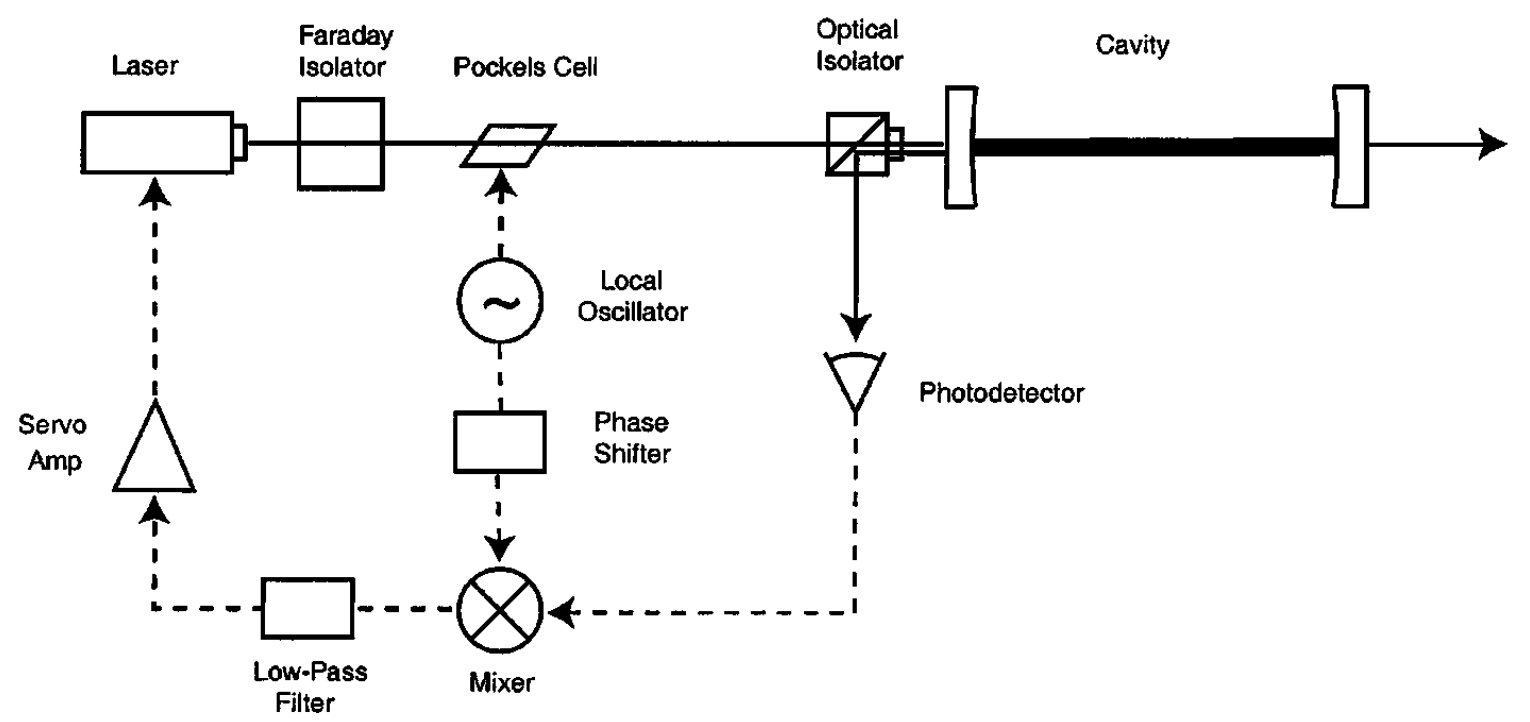
\includegraphics[width=.8\textwidth]{PDHlayout.png}
    \caption{The basic layout for locking a cavity to a laser. Solid lines are optical paths and dashed lines are signal paths. The signal going to the laser controls its frequency \cite{PDHintro}}
    \label{fig:PDHlayout}
\end{figure}

Referring to Fig \ref{fig:PDHlayout}, the basic steps of a PDH locking scheme is outlined as following: 
\begin{enumerate}
    \item A laser beam is passed through a Pockels cell to modulate its frequency at a frequency small relative to the $\Delta \nu_{fsr}$ free spectral range of the optical cavity. My cavity has length $L=15$cm, $\Delta \nu_{fsr} = c/2L \approx 1GHz$. Hence my EOM at $\approx 38 MHz$, as discussed in the EOM section, is appropriate here. Note that EOM only modulates light of polarisation parrallel to the EOM's oscillating electric field. In my case horizontal polarisation w.r.t the optical table is used. (i.e. a quarter-wave-plate and half-wave-plate pair is used to clean up laser beam polarisation to be horizontal before entering the EOM) 

    \item The beam goes do the cavity. An optical isolator is used to pick up reflected beam from the cavity. I used a quarter wave plate and a polarising beam splitter. 

    \item Referring to Fig \ref{fig:cavityTransmission}, if length of the cavity is set to one side of these resonances, but near enough that some light gets transmitted, then a small change in laser frequency would produce a proportional change in the transmitted intensity. Equivalently there will be a change in the reflected beam intensity. Optimising for minimum reflection has the following benefits over optimising for maximum transmission: 
    \begin{enumerate}
        \item Effect of laser frequency drift and intensity drift is decoupled due to obvious reason.
        \item The frequency of frequency drift that can be corrected for is not restricted by the cavity response time. As when measuring transmission intensity, it takes time for the fields in the cavity to re-equilibrate whenever there is frequency drift. Whereas measuring reflected intensity circumvents this issue. 
    \end{enumerate}

    \item In order to have a control loop that locks the laser to a certain frequency, we need an error signal that tells provides a $\pm$ sign for the feedback signal on top of the amplitude as given by the last point. To obtain an error signal, the EOM comes into play in that it varies the laser frequency slightly (small w.r.t cavity free spectral range as discussed earlier), indicating whether laser frequency is currently on the right side or left side of resonance. 

    \item What's left is to produce an error signal by using a fast photodiode (fast enough to discern MHz level modulation) to read beam intensity coming from the optical isolator. Signal from the fast photodiode is then processed as shown in Fig \ref{fig:PDHlayout}. For details on how the multiplicative mixer and the phase shifter helps output an error signal, see \cite{PDHintro}.

    \item Caution: Note that wave plates and polarising beam splitter are wavelength rated
\end{enumerate}

%TODO: insert image of my setup here
%TODo: insert image of error signal here

\subsection{Measuring Water Vapor concentration Using the PDH Setup}
Discuss: I am not doing the laser lock, but instead locking the cavity length to the frequency stable 738nm laser and measuring intensity drift due to water vapor change (as 935nm is readily absorbed by water) of the frequency-stable 935nm laser to indicate a water vapor concentration drift. 

\section{Other Discussions}
\subsection{General Optical Lab Techniques and devices}
\begin{enumerate}
    \item discuss various optical devices on the optical table (reference QDevice content): wave plates, polarisers, etc -> briefly on how they work + how to use them in the lab 
    \begin{enumerate}
        \item wave plates, polarisers
        \item AR coating
        \item laser power meter: wavelength selection -> response curve
        \item lens cleaning
        \item DIY relevant tools in the lab. exmaples: strips of paper for ray tracing
        \item electronics stuff: soldering, PCB board inspection
        
    \end{enumerate}
\end{enumerate}




\section{Conclusion}
\begin{enumerate}
    \item what have I learn: about theory and experimental physics lab
    \item what have I done 
    \item possible follow up investigations / improvement on existing current
\end{enumerate}

\section{Acknowledgements}
thank the lab people! Jaren, Muyoung, Dzmitry, Nigel, Kowei

\section{Appendix}
\begin{figure}[H]
    \centering
    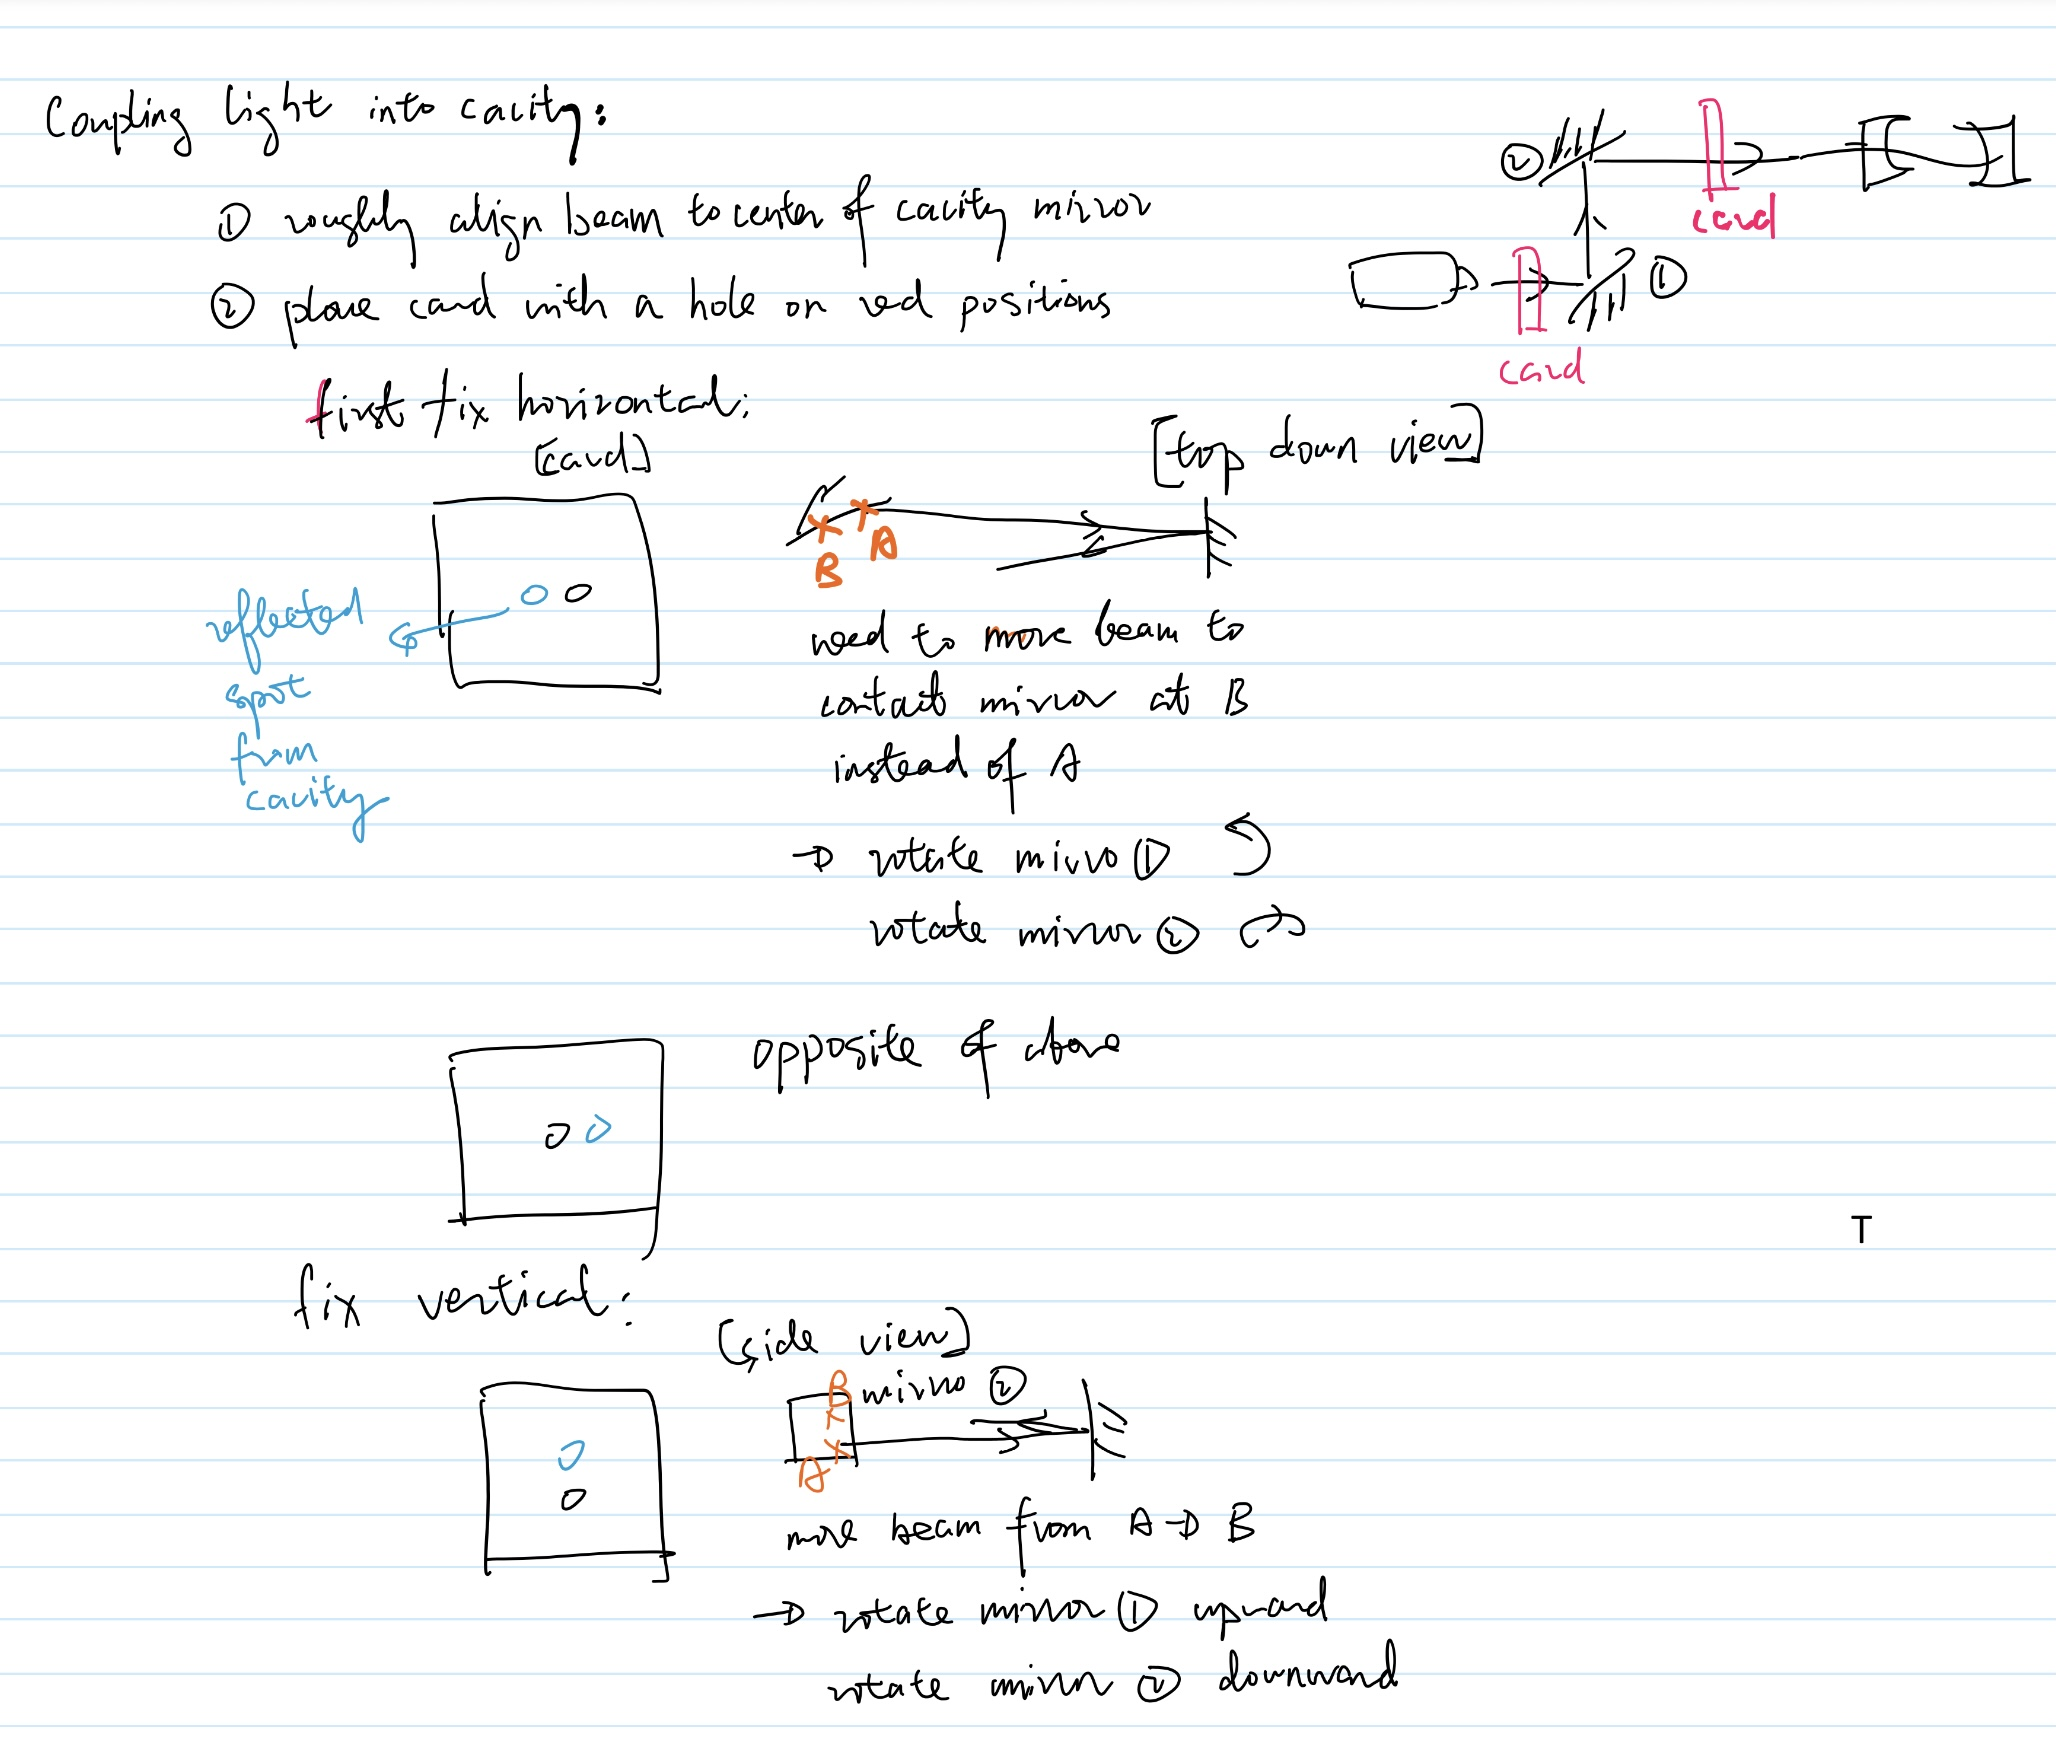
\includegraphics[width=\textwidth]{laserCavityCoupling.jpg}
    \caption{Laser beam - Cavity Coupling Note}
    \label{fig:laserCavityCoupling}
\end{figure}


\bibliographystyle{plain}
\bibliography{bibliography.bib}

\end{document}
